\documentclass{beamer}

% xcolor and define colors -------------------------
\usepackage{xcolor}

% https://www.viget.com/articles/color-contrast/
\definecolor{purple}{HTML}{5601A4}
\definecolor{navy}{HTML}{0D3D56}
\definecolor{ruby}{HTML}{9a2515}
\definecolor{alice}{HTML}{107895}
\definecolor{daisy}{HTML}{EBC944}
\definecolor{coral}{HTML}{F26D21}
\definecolor{kelly}{HTML}{829356}
\definecolor{cranberry}{HTML}{E64173}
\definecolor{jet}{HTML}{131516}
\definecolor{asher}{HTML}{555F61}
\definecolor{slate}{HTML}{314F4F}

% Mixtape Sessions
\definecolor{picton-blue}{HTML}{00b7ff}
\definecolor{violet-red}{HTML}{ff3881}
\definecolor{sun}{HTML}{ffaf18}
\definecolor{electric-violet}{HTML}{871EFF}

% Main theme colors
\definecolor{accent}{HTML}{00b7ff}
\definecolor{accent2}{HTML}{871EFF}
\definecolor{gray100}{HTML}{f3f4f6}
\definecolor{gray800}{HTML}{1F292D}


% Beamer Options -------------------------------------

% Background
\setbeamercolor{background canvas}{bg = white}

% Change text margins
\setbeamersize{text margin left = 15pt, text margin right = 15pt} 

% \alert
\setbeamercolor{alerted text}{fg = accent2}

% Frame title
\setbeamercolor{frametitle}{bg = white, fg = jet}
\setbeamercolor{framesubtitle}{bg = white, fg = accent}
\setbeamerfont{framesubtitle}{size = \small, shape = \itshape}

% Block
\setbeamercolor{block title}{fg = white, bg = accent2}
\setbeamercolor{block body}{fg = gray800, bg = gray100}

% Title page
\setbeamercolor{title}{fg = gray800}
\setbeamercolor{subtitle}{fg = accent}

%% Custom \maketitle and \titlepage
\setbeamertemplate{title page}
{
    %\begin{centering}
        \vspace{20mm}
        {\Large \usebeamerfont{title}\usebeamercolor[fg]{title}\inserttitle}\\
        {\large \itshape \usebeamerfont{subtitle}\usebeamercolor[fg]{subtitle}\insertsubtitle}\\ \vspace{10mm}
        {\insertauthor}\\
        {\color{asher}\small{\insertdate}}\\
    %\end{centering}
}

% Table of Contents
\setbeamercolor{section in toc}{fg = accent!70!jet}
\setbeamercolor{subsection in toc}{fg = jet}

% Button 
\setbeamercolor{button}{bg = accent}

% Remove navigation symbols
\setbeamertemplate{navigation symbols}{}

% Table and Figure captions
\setbeamercolor{caption}{fg=jet!70!white}
\setbeamercolor{caption name}{fg=jet}
\setbeamerfont{caption name}{shape = \itshape}

% Bullet points

%% Fix left-margins
\settowidth{\leftmargini}{\usebeamertemplate{itemize item}}
\addtolength{\leftmargini}{\labelsep}

%% enumerate item color
\setbeamercolor{enumerate item}{fg = accent}
\setbeamerfont{enumerate item}{size = \small}
\setbeamertemplate{enumerate item}{\insertenumlabel.}

%% itemize
\setbeamercolor{itemize item}{fg = accent!70!white}
\setbeamerfont{itemize item}{size = \small}
\setbeamertemplate{itemize item}[circle]

%% right arrow for subitems
\setbeamercolor{itemize subitem}{fg = accent!60!white}
\setbeamerfont{itemize subitem}{size = \small}
\setbeamertemplate{itemize subitem}{$\rightarrow$}

\setbeamertemplate{itemize subsubitem}[square]
\setbeamercolor{itemize subsubitem}{fg = jet}
\setbeamerfont{itemize subsubitem}{size = \small}







% Links ----------------------------------------------

\usepackage{hyperref}
\hypersetup{
  colorlinks = true,
  linkcolor = accent2,
  filecolor = accent2,
  urlcolor = accent2,
  citecolor = accent2,
}


% Line spacing --------------------------------------
\usepackage{setspace}
\setstretch{1.2}


% \begin{columns} -----------------------------------
\usepackage{multicol}


% Fonts ---------------------------------------------
% Beamer Option to use custom fonts
\usefonttheme{professionalfonts}

% \usepackage[utopia, smallerops, varg]{newtxmath}
% \usepackage{utopia}
\usepackage[sfdefault,light]{roboto}

% Small adjustments to text kerning
\usepackage{microtype}



% Remove annoying over-full box warnings -----------
\vfuzz2pt 
\hfuzz2pt


% Table of Contents with Sections
\setbeamerfont{myTOC}{series=\bfseries, size=\Large}
\AtBeginSection[]{
        \frame{
            \frametitle{Roadmap}
            \tableofcontents[current]   
        }
    }


% Tables -------------------------------------------
% Tables too big
% \begin{adjustbox}{width = 1.2\textwidth, center}
\usepackage{adjustbox}
\usepackage{array}
\usepackage{threeparttable, booktabs, adjustbox}
    
% Fix \input with tables
% \input fails when \\ is at end of external .tex file
\makeatletter
\let\input\@@input
\makeatother

% Tables too narrow
% \begin{tabularx}{\linewidth}{cols}
% col-types: X - center, L - left, R -right
% Relative scale: >{\hsize=.8\hsize}X/L/R
\usepackage{tabularx}
\newcolumntype{L}{>{\raggedright\arraybackslash}X}
\newcolumntype{R}{>{\raggedleft\arraybackslash}X}
\newcolumntype{C}{>{\centering\arraybackslash}X}

% Figures

% \imageframe{img_name} -----------------------------
% from https://github.com/mattjetwell/cousteau
\newcommand{\imageframe}[1]{%
    \begin{frame}[plain]
        \begin{tikzpicture}[remember picture, overlay]
            \node[at = (current page.center), xshift = 0cm] (cover) {%
                \includegraphics[keepaspectratio, width=\paperwidth, height=\paperheight]{#1}
            };
        \end{tikzpicture}
    \end{frame}%
}

% subfigures
\usepackage{subfigure}


% Highlight slide -----------------------------------
% \begin{transitionframe} Text \end{transitionframe}
% from paulgp's beamer tips
\newenvironment{transitionframe}{
    \setbeamercolor{background canvas}{bg=accent!40!black}
    \begin{frame}\color{accent!10!white}\LARGE\centering
}{
    \end{frame}
}


% Table Highlighting --------------------------------
% Create top-left and bottom-right markets in tabular cells with a unique matching id and these commands will outline those cells
\usepackage[beamer,customcolors]{hf-tikz}
\usetikzlibrary{calc}
\usetikzlibrary{fit,shapes.misc}

% To set the hypothesis highlighting boxes red.
\newcommand\marktopleft[1]{%
    \tikz[overlay,remember picture] 
        \node (marker-#1-a) at (0,1.5ex) {};%
}
\newcommand\markbottomright[1]{%
    \tikz[overlay,remember picture] 
        \node (marker-#1-b) at (0,0) {};%
    \tikz[accent!80!jet, ultra thick, overlay, remember picture, inner sep=4pt]
        \node[draw, rectangle, fit=(marker-#1-a.center) (marker-#1-b.center)] {};%
}

\usepackage{breqn} % Breaks lines

\usepackage{amsmath}
\usepackage{mathtools}

\usepackage{pdfpages} % \includepdf

\usepackage{listings} % R code
\usepackage{verbatim} % verbatim

% Video stuff
\usepackage{media9}

% packages for bibs and cites
\usepackage{natbib}
\usepackage{har2nat}
\newcommand{\possessivecite}[1]{\citeauthor{#1}'s \citeyearpar{#1}}
\usepackage{breakcites}
\usepackage{alltt}

% tikz
\usepackage{tikz}
\usepackage{pgfplots}
\usetikzlibrary{calc, positioning, decorations.pathreplacing, arrows.meta, intersections}
\pgfdeclarelayer{bg}
\pgfdeclarelayer{back}
\pgfdeclarelayer{fg}
\pgfsetlayers{bg,main,fg,back}
\usetikzlibrary{shapes,arrows}

% Setup math operators
\DeclareMathOperator{\E}{E} \DeclareMathOperator{\tr}{tr} \DeclareMathOperator{\se}{se} \DeclareMathOperator{\I}{I} \DeclareMathOperator{\sign}{sign} \DeclareMathOperator{\supp}{supp} \DeclareMathOperator{\plim}{plim}
\DeclareMathOperator*{\dlim}{\mathnormal{d}\mkern2mu-lim}
\newcommand\independent{\protect\mathpalette{\protect\independenT}{\perp}}
   \def\independenT#1#2{\mathrel{\rlap{$#1#2$}\mkern2mu{#1#2}}}
\newcommand*\colvec[1]{\begin{pmatrix}#1\end{pmatrix}}

\newcommand{\myurlshort}[2]{\href{#1}{\textcolor{gray}{\textsf{#2}}}}


\begin{document}

\imageframe{./lecture_includes/mixtape_ci_cover.png}


% ---- Content ----
\section{Randomization inference}

\subsection{Lady tasting tea}

\begin{frame}{Randomization inference and causal inference}

\begin{itemize}
\item ``In randomization-based inference, uncertainty in estimates arises naturally from the random assignment of the treatments, rather than from hypothesized sampling from a large population.'' (Athey and Imbens 2017)

\item Athey and Imbens is part of growing trend of economists using randomization-based methods for doing causal inference

\item Unclear (to me) why we are hearing more and more about randomization inference, but we are. 

\item Could be due to improved computational power and/or the availability of large data instead of samples?

\end{itemize}


\end{frame}




\begin{frame}{Lady tasting tea experiment}

	\begin{itemize}
	\item Ronald Aylmer Fisher (1890-1962)
		\begin{itemize}
		\item Two classic books on statistics: \emph{Statistical Methods for Research Workers} (1925) and \emph{The Design of Experiments} (1935), as well as a famous work in genetics, \emph{The Genetical Theory of Natural Science}
		\item Developed many fundamental notions of modern statistics including the theory of randomized experimental design.
		\end{itemize}

	\end{itemize}
	
\end{frame}


\begin{frame}{Lady tasting tea}

\begin{itemize}
	\item Muriel Bristol (1888-1950)
		\begin{itemize}
		\item A PhD scientist back in the days when women weren't PhD scientists
		\item Worked with Fisher at the Rothamsted Experiment Station (which she established) in 1919 
		\item During afternoon tea, Muriel claimed she could tell from taste whether the milk was added to the cup before or after the tea
		\item Scientists were incredulous, but Fisher was inspired by her strong claim
		\item He devised a way to test her claim which she passed using randomization inference
		\end{itemize}
\end{itemize}

\end{frame}

\begin{frame}{Description of the tea-tasting experiment}

	\begin{itemize}
	\item Original claim: Given a cup of tea with milk, Bristol claims she can discriminate the order in which the milk and tea were added to the cup
	\item Experiment: To test her claim, Fisher prepares 8 cups of tea -- 4 \textbf{milk then tea} and 4 \textbf{tea then milk} -- and presents each cup to Bristol for a taste test
	\item Question: How many cups must Bristol correctly identify to convince us of her unusual ability to identify the order in which the milk was poured?
	\item Fisher's sharp null: Assume she can't discriminate.  Then what's the likelihood that random chance was responsible for her answers?
	\end{itemize}
\end{frame}

\begin{frame}{Choosing subsets}
	
	\begin{itemize}
	\item The lady performs the experiment by selecting $4$ cups, say, the ones she claims to have had the tea poured first.
	 $${n \choose k} = \frac{n!}{k!(n-k)!}$$
	\item ``8 choose 4'' -- $ 8 \choose 4 $ -- ways to choose 4 cups out of 8
		
		\begin{itemize}
		\item Numerator is $8\times{7}\times{6}\times{5}=1,680$ ways to choose a first cup, a second cup, a third cup, and a fourth cup, in order.
		\item Denominator is $4\times{3}\times{2}\times{1}=24$ ways to order $4$ cups.
		\end{itemize}
	\end{itemize}
\end{frame}


\begin{frame}{Choosing subsets}

\begin{itemize}
	\item There are $70$ ways to choose $4$ cups out of $8$, and therefore a 1.4\% probability of producing the correct answer by chance
		\begin{eqnarray*}
		\frac{24}{1680}=1/70=0.014.
		\end{eqnarray*}
	\item For example, the probability that she would correctly identify all $4$ cups is $\frac{1}{70}$ 
\end{itemize}

\end{frame}


%\begin{frame}[plain]

%	\begin{center}
%	\textbf{Choosing $3$}
%	\end{center}
	
%	\begin{itemize}
%	\item To get exactly $3$ right, and, hence, $1$ wrong, she would have to choose $3$ from the $4$ correct ones.
%		\begin{enumerate}
%		\item She can do this by $4\times{3}\times{2}=24$ with order.
%		\item Since $3$ cups can be ordered in $3\times{2}=6$ ways, there are $4$ ways for her to choose the $3$ correctly.
%		\end{enumerate}
%	\item Since she can now choose the $1$ incorrect cup $4$ ways, there are a total of $4\times{4}=16$ ways for her to choose exactly $3$ right and $1$ wrong.
%	\item Hence the probability that she chooses exactly 3 correctly is $\frac{16}{70}=0.23$.
%	\end{itemize}
%\end{frame}

\begin{frame}{Statistical significance}
	
	\begin{itemize}
	\item Suppose the lady correctly identifies all 4 cups.  Then \dots
		\begin{enumerate}
		\item Either she has no ability, and has chosen the correct 4 cups purely by chance, or
		\item She has the discriminatory ability she claims.
		\end{enumerate}
	\item Since choosing correctly is highly unlikely in the first case (one chance in $70$), the second seems plausible.
	\item Bristol actually got all four correct
	\item I wonder if seeing this, any of the scientists present changed their mind
	\end{itemize}
\end{frame}

\subsection{Fisher's sharp null}

\begin{frame}{Null hypothesis}
	
	\begin{itemize}
	\item In this example, the null hypothesis is the hypothesis that the lady has no special ability to discriminate between the cups of tea.
	\item We can never prove the null hypothesis, but the data may provide evidence to reject it.
	\item In most situations, rejecting the null hypothesis is what we hope to do.

	\end{itemize}
\end{frame}



\begin{frame}{Null hypothesis of no effect}

\begin{itemize}
\item Randomization inference allows us to make probability calculations revealing whether the treatment assignment was ``unusual''
\item Fisher's sharp null is when entertain the possibility that no unit has a treatment effect
\item This allows us to make ``exact'' p-values which do not depend on large sample approximations
\item It also means the inference is not dependent on any particular distribution (e.g., Gaussian); sometimes called nonparametric
\end{itemize}

\end{frame}




\begin{frame}{Sidebar: bootstrapping is different}

\begin{itemize}
\item Sometimes people confuse randomization inference with bootstrapping
\item Bootstrapping randomly draws a percent of the total observations for estimation; ``uncertainty over the sample''
\item Randomization inference randomly reassigns the treatment;  ``uncertainty over treatment assignment''
\end{itemize}(Thanks to Jason Kerwin for helping frame the two against each other)

\end{frame}


\begin{frame}{6-step guide to randomization inference}

\begin{enumerate}
\item Choose a sharp null hypothesis (e.g., no treatment effects)
\item Calculate a test statistic ($T$ is a scalar based on $D$ and $Y$)
\item Then pick a randomized treatment vector $\tilde{D_1}$
\item Calculate the test statistic associated with $(\tilde{D},Y)$
\item Repeat steps 3 and 4 for all possible combinations to get $\tilde{T} = \{\tilde{T}_1, \dots , \tilde{T}_K \}$
\item Calculate exact p-value as $p=\frac{1}{K} \sum_{k=1}^K I(\tilde{T}_k \geq T)$
\end{enumerate}
\end{frame}


\begin{frame}{Pretend experiment}

\begin{table}[htbp]\centering
\begin{center}
\caption{Pretend DBT intervention for some homeless population}
\begin{threeparttable}
\begin{tabular}{lcccc}
\toprule
\multicolumn{1}{l}{Name}&
\multicolumn{1}{c}{D}&
\multicolumn{1}{c}{Y}&
\multicolumn{1}{c}{Y$^0$}&
\multicolumn{1}{c}{Y$^1$}\\
\midrule
Andy		& 1 & 10  & . & 10 \\
Ben		& 1 & 5    & . & 5 \\
Chad	& 1 & 16  & . & 16 \\	
Daniel	& 1 &  3   & . & 3 \\
Edith		& 0 & 5    & 5 & . \\
Frank	& 0 & 7    & 7&.  \\
George	& 0 & 8    & 8 & . \\
Hank		& 0 & 10  & 10 & . \\
\bottomrule
\end{tabular}
\end{threeparttable}
\end{center}
\end{table}

For concreteness, assume a program where we pay homeless people \$15 to take dialectical behavioral therapy (DBT). Outcomes are some measure of mental health 0-20 with higher scores being improvements in mental health symptoms. 
	
\end{frame}



\begin{frame}{Step 1: Sharp null of no effect}

\begin{block}{Fisher's Sharp Null Hypothesis}
$H_0: \delta_i = Y_i^1 - Y_i^0 = 0 \text{ } \forall i$
\end{block}

\begin{itemize}
\item Assuming no effect means any test statistic is due to chance
\item Neyman and Fisher test statistics were different -- Fisher was exact, Neyman was not
\item Neyman's null was no average treatment effect (ATE=0). If you have a treatment effect of 5 and I have a treatment effect of -5, our ATE is zero. This is not the sharp null even though it also implies a zero ATE

\end{itemize}

\end{frame}


\begin{frame}{More sharp null}

\begin{itemize}
\item Since under the Fisher sharp null $\delta_i=0$, it means each unit's potential outcomes under both states of the world are the same
\item We therefore know each unit's missing counterfactual
\item The randomization we will perform will cycle through all treatment assignments under a null well treatment assignment doesn't matter because all treatment assignments are associated with a null of zero unit treatment effects
\item We are looking for evidence \emph{against} the null 
\end{itemize}

\end{frame}




\begin{frame}{Step 1: Fisher's sharp null and missing potential outcomes}

\begin{table}[htbp]\centering
\begin{center}
\caption{Missing potential outcomes are no longer missing}
\begin{threeparttable}
\begin{tabular}{lcccc}
\toprule
\multicolumn{1}{l}{Name}&
\multicolumn{1}{c}{D}&
\multicolumn{1}{c}{Y}&
\multicolumn{1}{c}{Y$^0$}&
\multicolumn{1}{c}{Y$^1$}\\
\midrule
Andy		& 1 & 10  & \textbf{10} & 10 \\
Ben		& 1 & 5    & \textbf{5} & 5 \\
Chad	& 1 & 16  & \textbf{16} & 16 \\	
Daniel	& 1 &  3   & \textbf{3} & 3 \\
Edith		& 0 & 5    & 5 & \textbf{5} \\
Frank	& 0 & 7    & 7& \textbf{7}  \\
George	& 0 & 8    & 8 & \textbf{8} \\
Hank		& 0 & 10  & 10 & \textbf{10} \\
\bottomrule
\end{tabular}
\end{threeparttable}
\end{center}
\end{table}

Fisher sharp null allows us to \textbf{fill in} the missing counterfactuals bc under the null there's zero treatment effect at the unit level.
	
\end{frame}

\begin{frame}{Step 2: Choosing a test statistic}

\begin{block}{Test Statistic}
A test statistic $T(D,Y)$ is a scalar quantity calculated from the treatment assignments  $D$ and the observed outcomes $Y$ 
\end{block}

\begin{itemize}
\item By scalar, I just mean it's a number (vs. a function) measuring some relationship between $D$ and $Y$
\item Ultimately there are many tests to choose from; I'll review a few later
\item If you want a test statistic with high statistical power, you need large values when the null is false, and small values when the null is true (i.e., \emph{extreme})
\end{itemize}

\end{frame}

\begin{frame}{Simple difference in means}

\begin{itemize}
\item Consider the absolute SDO from earlier $$ \delta_{SDO} = \bigg | \frac{1}{N_T} \sum_{i=1}^N D_iY_i - \frac{1}{N_C} \sum_{i=1}^N (1-D_i)Y_i \bigg |$$
\item Larger values of $\delta_{SDO}$ are evidence \emph{against} the sharp null
\item Good estimator for constant, additive treatment effects and relatively few outliers in the potential outcomes
\end{itemize}

\end{frame}

\begin{frame}{Step 2: Calculate test statistic, $T(D,Y)$}

\begin{table}[htbp]\centering
\begin{center}
\caption{Calculate $T$ using $D$ and $Y$}
\begin{threeparttable}
\begin{tabular}{lccccc}
\toprule
\multicolumn{1}{l}{Name}&
\multicolumn{1}{c}{D}&
\multicolumn{1}{c}{Y}&
\multicolumn{1}{c}{Y$^0$}&
\multicolumn{1}{c}{Y$^1$}&
\multicolumn{1}{c}{$\delta_i$}\\
\midrule
Andy		& \textbf{1} & \textbf{10}  & {10} & {10} & 0\\
Ben		& \textbf{1} & \textbf{5}    & {5} & {5} & 0 \\
Chad	& \textbf{1} & \textbf{16}  & {16} & {16} & 0 \\	
Daniel	& \textbf{1} &  \textbf{3}   & {3} & {3} & 0 \\
Edith		& \textbf{0} & \textbf{5}    & {5} & {5} & 0 \\
Frank	& \textbf{0} & \textbf{7}    & {7} & {7} & 0  \\
George	& \textbf{0} &\textbf {8}    & {8} & {8} & 0 \\
Hank		& \textbf{0} & \textbf{10}  & {10} & {10} & 0 \\
\bottomrule
\end{tabular}
\end{threeparttable}
\end{center}
\end{table}

We'll start with this simple the simple difference in means test statistic, $T(D,Y)$: $\delta_{SDO} = 34/4 - 30/4 = 1$	
\end{frame}



\begin{frame}{Steps 3-5: Null randomization distribution}

\begin{itemize}
\item Randomization steps reassign treatment assignment for every combination, calculating test statistics each time, to obtain the entire distribution of counterfactual test statistics
\item The key insight of randomization inference is that under Fisher's sharp null, the treatment assignment shouldn't matter
\item Ask yourself: 
	\begin{itemize}
	\item if there is no unit level treatment effect, can you picture a distribution of counterfactual test statistics?
	\item and if there is no unit level treatment effect, what must average counterfactual test statistics equal?
	\end{itemize}
\end{itemize}

\end{frame}

\begin{frame}{Step 6: Calculate ``exact'' p-values}

\begin{itemize}
\item Question: how often would we get a test statistic as big or bigger as our ``real'' one if Fisher's sharp null was true?
\item This can be calculated ``easily'' (sometimes) once we have the randomization distribution from steps 3-5
	\begin{itemize}
	\item The number of test statistics ($t(D,Y)$) bigger than the observed divided by total number of randomizations $$Pr(T(D,Y) \geq T(\tilde{D},Y | \delta = 0)) = \frac{ \sum_{D \in \Omega} I(T(D,Y) \leq T(\tilde{D},Y)}{K}$$
	\end{itemize}
\end{itemize}
\end{frame}


%\begin{frame}[plain]

%\begin{center}
%\textbf{Simulation}
%\end{center}

%Download the file \texttt{combinations.do} and you can do this yourself for this dataset of eight people.  It will do exact combinations. 

%\end{frame}


\begin{frame}{First permutation (holding $N_T$ fixed)}

\begin{table}[htbp]\centering
\begin{center}
\begin{threeparttable}
\begin{tabular}{lcccc}
\toprule
\multicolumn{1}{l}{Name}&
\multicolumn{1}{c}{$\tilde{D_2}$}&
\multicolumn{1}{c}{Y}&
\multicolumn{1}{c}{Y$^0$}&
\multicolumn{1}{c}{Y$^1$}\\
Andy		& 1 & \textcolor{blue}{10}  & {10} & 10 \\
Ben		& 0 & \textcolor{red}{5}    & {5} & 5 \\
Chad	& 1 & \textcolor{blue}{16}  & {16} & 16 \\	
Daniel	& 1 &  \textcolor{blue}{3}   & {3} & 3 \\
Edith		& 0 & \textcolor{red}{5}    & 5 & {5} \\
Frank	& 1 & \textcolor{blue}{7}    & 7& {7}  \\
George	& 0 & \textcolor{red}{8}    & 8 & {8} \\
Hank		& 0 & \textcolor{red}{10}  & 10 & {10} \\
\bottomrule
\end{tabular}
\end{threeparttable}
\end{center}
\end{table}

$$\tilde{T}_1 =  | \textcolor{blue}{36/4} - \textcolor{red}{28/4}  | = \textcolor{blue}{9} - \textcolor{red}{7} = 2$$
	
\end{frame}

\begin{frame}{Second permutation (again holding $N_T$ fixed)}

\begin{table}[htbp]\centering
\begin{center}
\begin{threeparttable}
\begin{tabular}{lcccc}
\toprule
\multicolumn{1}{l}{Name}&
\multicolumn{1}{c}{$\tilde{D_3}$}&
\multicolumn{1}{c}{Y}&
\multicolumn{1}{c}{Y$^0$}&
\multicolumn{1}{c}{Y$^1$}\\
Andy		& 1 & \textcolor{blue}{10}  & {10} & 10 \\
Ben		& 0 & \textcolor{red}{5}    & {5} & 5 \\
Chad	& 1 & \textcolor{blue}{16}  & {16} & 16 \\	
Daniel	& 1 &  \textcolor{blue}{3}   & {3} & 3 \\
Edith		& 0 & \textcolor{red}{5}    & 5 & {5} \\
Frank	& 0 & \textcolor{red}{7}    & 7& {7}  \\
George	& 1 & \textcolor{blue}{8}    & 8 & {8} \\
Hank		& 0 & \textcolor{red}{10}  & 10 & {10} \\
\bottomrule
\end{tabular}
\end{threeparttable}
\end{center}
\end{table}

$$T_{rank} =  | \textcolor{blue}{36/4} - \textcolor{red}{27/4}  | = \textcolor{blue}{9} - \textcolor{red}{6.75} = 2.25$$
	
\end{frame}

\begin{frame}{Sidebar: Should it be 4 treatment groups each time?}

\begin{itemize}
\item In this experiment, I've been using the same $N_T$ \emph{under the assumption} that $N_T$ had been fixed when the experiment was drawn.
\item But if the original treatment assignment had been generated by something like a Bernoulli distribution (e.g., coin flips over every unit), then you should be doing a complete permutation that is also random in this way
\item This means that for 8 units, sometimes you'd have 1 treated, or even 8
\item Correct inference requires you know the original data generating process
\end{itemize}

\end{frame}

\begin{frame}{Randomization distribution}

\begin{table}[htbp]\centering
\begin{center}
\begin{threeparttable}
\begin{tabular}{lccccccccc}
\toprule
\multicolumn{1}{l}{Assignment}&
\multicolumn{1}{c}{$D_1$}&
\multicolumn{1}{c}{$D_2$}&
\multicolumn{1}{c}{$D_3$}&
\multicolumn{1}{c}{$D_4$}&
\multicolumn{1}{c}{$D_5$}&
\multicolumn{1}{c}{$D_6$}&
\multicolumn{1}{c}{$D_7$}&
\multicolumn{1}{c}{$D_8$}&
\multicolumn{1}{c}{$|T_i|$}\\
\midrule
True $D$ & 1 & 1 & 1 & 1 & 0 & 0 & 0 & 0 & 1 \\
$\tilde{D_2}$ & 1 & 0 & 1 & 1 & 0 & 1 & 0 & 0 & 2 \\
$\tilde{D_3}$ & 1 & 0 & 1 & 1 & 0 & 0 & 1 & 0 & 2.25 \\
\dots \\
\bottomrule
\end{tabular}
\end{threeparttable}
\end{center}
\end{table}

\end{frame}

\subsection{Alternative test statistics}

\begin{frame}{Step 2: Other test statistics}

\begin{itemize}
\item The simple difference in means is fine when effects are additive, and there are few outliers in the data
\item But outliers create more variation in the randomization distribution
\item A good test statistic is the one that best fits your data.  
\item Some test statistics will have weird properties in the randomization as we'll see in synthetic control.
\item What are some alternative test statistics?
\end{itemize}

\end{frame}

\begin{frame}{Transformations}

\begin{itemize}
\item What if there was a constant multiplicative effect: $Y_i^1 / Y_i^0 = C$?
\item Difference in means will have low power to detect this alternative hypothesis
\item So we transform the observed outcome using the natural log:

$$T_{log} = \bigg | \frac{1}{N_T} \sum_{i=1}^N D_i ln(Y_i) - \frac{1}{N_C} \sum_{i=1}^N (1-D_i) ln(Y_i) \bigg |$$
\item This is useful for skewed distributions of outcomes

\end{itemize}

\end{frame}

\begin{frame}{Difference in medians/quantiles}

\begin{itemize}
\item We can protect against outliers using other test statistics such as the difference in quantiles
\item Difference in medians:$$T_{median} = | median(Y_T) - median(Y_C)|$$
\item We could also estimate the difference in quantiles at any point in the distribution (e.g., 25th or 75th quantile)
\end{itemize}

\end{frame}

\begin{frame}{Rank test statistics}

\begin{itemize}
\item Basic idea is rank the outcomes (higher values of $Y_i$ are assigned higher ranks) 
\item Then calculate a test statistic based on the transformed ranked outcome (e.g., mean rank)
\item Useful with continuous outcomes, small datasets and/or many outliers
\end{itemize}

\end{frame}

\begin{frame}{Rank statistics formally}

\begin{itemize}
\item Rank is the domination of others (including oneself): $$\tilde{R} = \tilde{R}_i(Y_1, \dots , Y_N) = \sum_{j=1}^N I(Y_j \leq Y_i)$$
\item Normalize the ranks to have mean 0 $$\tilde{R}_i = \tilde{R}_i(Y_1, \dots, Y_N) = \sum_{j=1}^N I(Y_j \leq Y_i) - \frac{N+1}{2}$$
\item Calculate the absolute difference in average ranks: $$T_{rank} = |\overline{R}_T - \overline{R}_C | = \bigg | \frac{\sum_{i:D_i=1} R_i}{N_T} - \frac{\sum_{i:D_i=0} R_i}{N_C} \bigg |$$
\item Minor adjustment (averages) for ties
\end{itemize}

\end{frame}

\begin{frame}{Randomization distribution}

\begin{table}[htbp]\centering
\begin{center}
\begin{threeparttable}
\begin{tabular}{l|cc|cc|cc}
\toprule
\multicolumn{1}{l}{Name}&
\multicolumn{1}{c}{D}&
\multicolumn{1}{c}{Y}&
\multicolumn{1}{c}{Y$^0$}&
\multicolumn{1}{c}{Y$^1$}&
\multicolumn{1}{c}{Rank}&
\multicolumn{1}{c}{$R_i$}\\
\midrule
Andy		& 1 & 10  & \textbf{10} & 10 & 6.5 & 2\\
Ben		& 1 & 5    & \textbf{5} & 5 & 2.5 & -2\\
Chad	& 1 & 16  & \textbf{16} & 16 & 8  &3.5 \\
Daniel	& 1 &  3   & \textbf{3} & 3 & 1 & -3.5\\
Edith		& 0 & 5    & 5 & \textbf{5} & 2.5 & -2\\
Frank	& 0 & 7    & 7& \textbf{7} & 4 & -0.5 \\
George	& 0 & 8    & 8 & \textbf{8} & 5 & 0.5\\
Hank		& 0 & 10  & 10 & \textbf{10} & 6.5 & 2\\
\bottomrule
\end{tabular}
\end{threeparttable}
\end{center}
\end{table}


$$T_{rank} = | 0 - 0 | = 0$$

\end{frame}

\begin{frame}{Effects on outcome distributions}

\begin{itemize}
\item Focused so far on ``average'' differences between groups.
\item Kolmogorov-Smirnov test statistics is based on the difference in the distribution of outcomes 
\item Empirical cumulative distribution function (eCDF): 
\begin{eqnarray*}
\widehat{F}_C(Y) &=& \frac{1}{N_C} \sum_{i:D_i=0} 1(Y_i \leq Y) \\
\widehat{F}_T(Y)&=& \frac{1}{N_T} \sum_{i:D_i=1} 1(Y_i \leq Y)
\end{eqnarray*}
\item Proportion of observed outcomes below a chosen value for treated and control separately
\item If two distributions are the same, then $\widehat{F}_C(Y) = \widehat{F}_T(Y)$
\end{itemize}

\end{frame}


\begin{frame}{Kolmogorov-Smirnov statistic}

\begin{itemize}
\item Test statistics are scalars not functions
\item eCDFs are functions, not scalars
\item Solution: use the maximum discrepancy between the two eCDFs:$$T_{KS} = max | \widehat{F}_T(Y_i) - \widehat{F}_C(Y_i) |$$
\end{itemize}

\end{frame}

\begin{frame}{eCDFs by treatment status and test statistic}

	\begin{figure}
	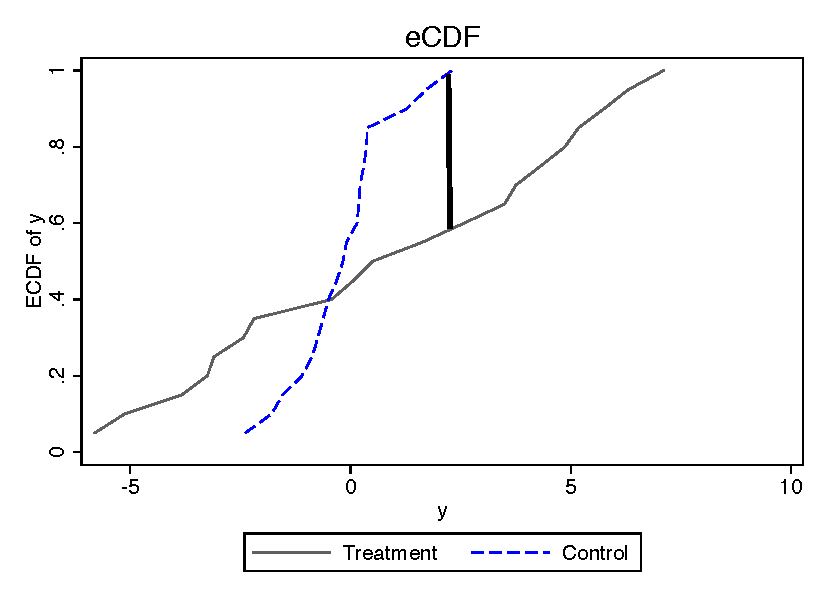
\includegraphics[scale=0.8]{./lecture_includes/ecdf.pdf}     
	\end{figure}
	
\end{frame}




\begin{frame}{Small vs. Modest Sample Sizes are non-trivial}

Computing the exact randomization distribution is not always feasible (Wolfram Alpha)
\begin{itemize}
\item $N=6$ and $N_T=3$ gives us 20 assignment vectors
\item $N=8$ and $N_T=4$ gives us 70 assignment vectors
\item $N=10$ and $N_T=5$ gives us 252 assignment vectors
\item $N=20$ and $N_T=10$ gives us 184,756 assignment vectors
\item $N=50$ and $N_T=25$ gives us 1.2641061$\times 10^{14}$ assignment vectors
\end{itemize}
Exact $p$ calculations are not realistic bc the number of assignments explodes at even modest size

\end{frame}



\begin{frame}{Approximate p-values}

These have been ``exact'' tests when they use every possible combination of $D$ 
	\begin{itemize}
	\item When you can't use every combination, then you can get \emph{approximate} p-values from a simulation (TBD)
	\item With a rejection threshold of $\alpha$ (e.g., 0.05), randomization inference test will falsely reject less than 100$\times \alpha$\% of the time
	\end{itemize}

\end{frame}
\begin{frame}{Approximate $p$ values}

\begin{itemize}
\item Use simulation to get approximate $p$-values
	\begin{itemize}
	\item Take $K$ samples from the treatment assignment space
	\item Calculate the randomization distribution in the $K$ samples
	\item Tests no longer exact, but bias is under your control (increase $K$)
	\end{itemize}
\item Imbens and Rubin show that $p$ values converge to stable $p$ values pretty quickly (in their example after 1000 replications)
\end{itemize}

\end{frame}


\begin{frame}{Thornton's experiment}

\begin{table}[htbp]\small\index{starrandom}
\centering
\begin{tabular}{lcccc}
\toprule
ATE & Iteration & Rank & $p$ & no. trials \\
\midrule
0.45 	 & 1 & 1 & 0.01 & 100\\
0.45 	 & 1 & 1 & 0.002 & 500\\
0.45 	 & 1 & 1 & 0.001 & 1000\\
\bottomrule
\end{tabular}
\caption{Estimated $p$-value using different number of trials.}
\label{tab:starrandom}
\end{table}

\end{frame}

\begin{frame}{Including covariate information}

\begin{itemize}
\item Let $X_i$ be a pretreatment measure of the outcome
\item One way is to use this as a gain score: $Y^{d'} = Y_i^d - X_i$
\item Causal effects are the same $Y^{1i} - Y^{0i} = Y_i^1 - Y_i^0$
\item But the test statistic is different:
\begin{eqnarray*}
T_{gain} = \bigg | ( \overline{Y}_T - \overline{Y}_C ) - (\overline{X}_T - \overline{X}_C ) \bigg |
\end{eqnarray*}
\item If $X_i$ is strongly predictive of $Y_i^0$, then this could have higher power
	\begin{itemize}
	\item $Y_{gain}$ will have lower variance under the null
	\item This makes it easier to detect smaller effects
	\end{itemize}
\end{itemize}

\end{frame}

\begin{frame}{Regression in RI}

\begin{itemize}
\item We can extend this to use covariates in more complicated ways
\item For instance, we can use an OLS regression:
\begin{eqnarray*}
Y_i = \alpha + \delta D_i + \beta X_i +  \varepsilon
\end{eqnarray*}
\item Then our test statistic could be $T_{OLS} = \widehat{\delta}$
\item RI is justified even if the model is wrong
	\begin{itemize}
	\item OLS is just another way to generate a test statistic
	\item The more the model is ``right'' (read: predictive of $Y_i^0$), the higher the power $T_{OLS}$ will have
	\end{itemize}
\item See if you can do this in Thornton's dataset using the loops and saving the OLS coefficient (or just use \texttt{ritest})
\end{itemize}

\end{frame}

\begin{frame}{Concluding remarks}

\begin{itemize}
\item Randomization inference is very common, particularly useful you don't want to make strong assumptions (parametric free)
\item It's an area of continual examination by statisticians and econometricians, both in the experimental design and the quasi-experimental design
\item We will use it primarily in my workshops with synthetic control, but it's going to be one you encounter and valued because of the non-parametric nature of it
\end{itemize}

\end{frame}



\end{document}


\begin{frame}{Angrist and Imbens and the 1990s}

  \begin{itemize}
    \item Angrist writes a dissertation using randomized instruments (Vietnam draft), goes to Harvard, overlaps with Imbens for a year, they are mentored by Gary Chamberlain, work with Don Rubin, write their famous LATE paper
    \item Chamberlain recommends potential outcomes framework over a different one that had been used at that time (latent index) and that seems to make the work more generally attractive (like to Rubin)
    \item Let's spend twenty minutes listening to them
  \end{itemize}

\end{frame}

\begin{frame}{Angrist, Imbens and Harvard}


  Josh Angrist on the negative results at the time (10 min)

  \url{https://youtu.be/ApNtXe-JDfA?t=1885}


  \bigskip
  Guido Imbens on the reception of their work (10 min)

  \url{https://youtu.be/cm8V65AS5iU?t=799}

\end{frame}
